\documentclass[a4paper,11pt]{article}
\usepackage{ifpdf}

\ifpdf
\usepackage[pdftex]{graphicx}
\usepackage[pdftex]{hyperref}
\else
\usepackage{graphicx}
\usepackage{hyperref}
\fi

\usepackage[svgnames]{xcolor}
\usepackage{minted}
\usepackage{amsmath}
\usepackage{amssymb}
\usepackage{xspace}
\usepackage{booktabs}
\usepackage{longtable}
\usepackage[top=3cm, bottom=3cm, left=2.5cm,right=2.5cm]{geometry}
%\usepackage[left=3cm,right=3cm]{geometry}

\pagestyle{headings}

\author{Stuart Moodie, Maciej Swat and Niels Kristensen}
\date{Aug 12, 2013}
\title{Proposed revision to Trail Design in \pharmml}

\colorlet{bkgd}{gray!5}
%\usemintedstyle{trac}

%\newminted{xml}{bgcolor=bkgd,fontsize=\footnotesize%
%,fontfamily=courier%
%}

\newminted{xml}{fontsize=\footnotesize,fontfamily=courier}

% \newcommand{\inputxml}[1]{\inputminted[bgcolor=bkgd,fontsize=\scriptsize%
% ,fontfamily=courier%
% ]{xml}{codesnippets/#1}}

\newcommand{\cellml}{CellML\xspace}
\newcommand{\sbml}{SBML\xspace}
\newcommand{\sedml}{SED-ML\xspace}
\newcommand{\mathml}{MathML\xspace}
\newcommand{\uncertml}{UncertML\xspace}
\newcommand{\pharmml}{PharmML\xspace}
\newcommand{\xelem}[1]{\texttt{<#1>}\index{XML Element!\texttt{<#1>}}}
\newcommand{\xatt}[1]{\texttt{#1}\index{XML Attribute!\texttt{#1}}}

\begin{document}

\maketitle

\tableofcontents

\section{Introduction}

This document contains a proposal to radically revise the way the
trial design and estimation steps are designed in the existing
\pharmml specification. The proposal has been discussed and agreed
between us and is our preferred way ahead. This document aims to set
out the problems with the current approach and then go on to propose,
what we think is a better solution.

\section{Fixing the problems in the Trial Design}

\subsection{The problems to be addressed}

In version 0.1 of the specification we provided 2 ways to define the
trial design. You could define the trial structure explicitly using
the \xelem{Design} element and its children or you could define the
trial design in the data file used to describe estimation or
simulation. The first approach has many virtues in that it explicitly
defines what is only implied by the data file approach, it is easy
to understand, non-redundant. The second approach is much less clear
since the dosing regiment, occasion structure, covariates and
objective data are all combined into a single tabular structure that
is inherently very redundant and much harder to understand. However,
the data-file approach is that adopted by tools such as NONMEM and
MONOLIX.

Both approaches, as implemented in the current version of \pharmml,
have limitations that we do need to address in a future release.

{\small%
\begin{longtable}{p{5cm} p{10cm}}\toprule
  \multicolumn{2}{l}{\textbf{Explicit Trial Design}}\\\midrule
  Occasions cannot span epochs. & Because an occasion is a child of an
  \xelem{TrialEpoch} element, it was not designed to span an epoch. It
  is desirable to do this however, so this needs hierarchy relationship
  needs to be re-examined.\\
  Higher levels of variability cannot be represent. & If one wants to
  represent variability between study centres, or countries and one
  wants to represent this variability as a random effect (and not use
  occasions) then \pharmml cannot do this currently.\\
  Washout and run-in periods are treated as epochs. & For consistency we
  should treat these as epochs and so enable occasions to span them.\\
  Varying bolus doses not supported. & It is not possible to define a
  dose amount that changes at each dosing time within a single Bolus
  dosing regimen. It would seem sensible to enable this.\\
  Per-individual doses not supported. & It is not possible to define a
  dose amount that changes per individual. If a dosing amount is
  per-body weight then this can be done in an equation, but you cannot
  currently specify a different absolute dose amount per subject.\\\\
  \multicolumn{2}{l}{\textbf{Design in Data-File}}\\\midrule
  Reading a data-file requires is imperative. & One of the main
  principles of \pharmml is that is declarative. However, the components
  in the estimation and simulation steps that define how a data file is
  read are inherently not. In particular the order that the line of the file
  is read in is significant. In some more complex trial designs there
  may be two or three lines describing the same time-point. Altering the
  order of these lines may, in pathological cases,  alter the result of
  the model.\\
  Easy to generate, difficult to convert to a target. & The current
  data-file structures in the estimation and simulation steps can be
  relatively generated from formats such as NMTRAN and MLXTRAN. However,
  there may be information loss because the \pharmml representation does
  not make any assumptions about the content of the data-file and so
  has to do more work.\\
  Some dosing regimens cannot be described. &  Some dosing regimens
  described in NONMEM cannot be handled by this approach. For example
  a repeated steady state infusion will have values in the
  columns TIME, DOSE, RATE, SS and II, which in combination have
  special meanings. In the current version it is not possible to use this information in the
  datafile to describe such a dosing regiment.\\
Typing of file contents. & Many of the values in a data file are
assigned to variables or parameters in the model. This means that they
should have types that match the element in the model. At present this
is undefined behaviour and the implication is that the item in the
file which be converted from a string to the appropriate
value. However, although this can be validated it is more work and as
with all implicit conversions there may cases where the conversion
made is incorrect. For example 'T' can be a string or a Boolean value for TRUE?\\
Defining possible values. & In come cases, such as defining the set of
individuals, or the possible categorical values for a categorical
covariate such information must be implied by the unique set of values
in the data file. This does not permit one to define categories in
your model, that are not used by the current population of
subjects. It is also potentially error prone. For example in a data
file you may have a set of 10 rows containing the same ID value. What
if the 5th row contains a different value? Is this a mistake or
intended? It's probably a mistake, but when using the contents to
describe the set of all possible values this kind of error cannot be
identified with certainty.\\
\bottomrule
\end{longtable}%
}
A final issue with the approach take in the current specification is
that we have 2 ways of doing the same thing, namely defining the trial
design. Which version should we recommend you use? Worse, they don't
have completely equivalent functionality. The issues associated with
maintaining two ways to do the same thing can be summarised as:
\begin{itemize}
\item It increases the complexity of the language making it harder to
  learn and to validate in software.
\item It increases the effort required to design and test the
  language and to bug fix. Naively, one would expect duplicate structures within the
  language to require double such effort.
\item Duplication also increases the work of converters because they
  now need to map two sets of \pharmml structures to the same target structures.
\item Ironically increased flexibility can make \pharmml harder to
  learn and be detrimental to adoption. Users are unclear which
  structures to use and would tend to want to avoid having to learn
  two ways to do the same thing.
\pharmml. 
\end{itemize}
%
So to conclude, I am advocating that whether we adopt my proposed
changes here, I would recommend that we stick with only one way of
defining the trial design in the next version of \pharmml.

\subsection{Outline of changes to the trial design}

From the critique above, it is inevitable that any changes I am
proposing must also affect the estimation and simulation step sections
of \pharmml. That is the case. In looking at the problem, it occurred
to me that the data-file conflates three classes of information:
\begin{description}
\item[Population] The attributes of the individuals in the study: the
  population in the population model. Each individual has a weight,
  an age, a gender and numerous other properties that may or may not
  be modelled as covariates in a given model. In addition, these
  properties may change over time.
\item[Dosing] When and how a drug or drugs are administered to the
  individuals in the trial.
\item[Measurements] These are the observations taken from each
  individual and specific times during the study. Such measurements
  provide the objective data used during parameter estimation and are
  typically the outputs calculated during a simulation.
\end{description}
Fortunately, I was not alone in this view and the developers of PharML\footnote{I'm not
  sure what the definitive reference of link is to the PharML spec
  is.} had this insight and developed this language accordingly.

By separating out these classes of information you can see that the
information we need to define the clinical trial is as follows:
\begin{description}
\item[Trial Structure] The organisation of the trial, how the subjects
  are grouped into different treatment groups and what the dosing
  regiment is within these treatment groups.
\item[Population] As above, the properties specific to the individual,
  including those that vary over time.
\item[Individual Dosing] This is related to the treatment regimens
  described in the trial structure, but describes the dosing of each
  subject in the study.
\end{description}

In essence my proposal is that we redesign the Design section of
\pharmml to handle the represent the information and that this is the
only place the trial design is defined in \pharmml. That way the
estimation step can be significantly simplified and it's main focus
can be the mapping of the objective data to the model and the
description of an estimation task.

\subsection{Proposed changes}

The first thing to note is that the \xelem{Design} element has been
renamed to \xelem{TrialDesign}. I think this is more consistent with
what we tend to call the information represented in this element. The
next things is the element \xelem{Structure}. This element is used to
define the structure of the trial. To do this I have reused, almost
verbatim, the CDISC Study Design Model\footnote{CDISC URL to go
  here.}, which is an XML representation of a clinical trial. Using
this design gives us the reassurance that we should be able to
represent all trial structures that we are likely to encounter.

The figure below (figure \ref{fig:cdiscstruct}) shows how the CDISC
trial structure is organised. It has five main components:
\begin{description}
\item[Epoch] The epoch defines a period of time during the study which
  has a purpose within the study. For example a washout or a treatment
  window. In CDISC Epochs can describe screening or follow-up periods,
  which are out of the scope of \pharmml. An epoch is usually defined
  by a time period.
\item[Arm] The arm represents a path through the study taken by a
  subject. An arm is composed of a study cell for each epoch in the study.
\item[Cell] The study cell describes what is carried out during an
  epoch in a particular arm. There is only one cell per epoch.
\item[Segment] The segment describes a set of planned observations and
  interventions, which may or may not involve treatment. Note that in
  \pharmml our definition is more limited and we only describe
  treatments. A segment can contains one or more activities.
\item[Activity] The activity is an action that is taken in the
  study. Here it is typically a treatment regimen.
\item[StudyEvent] A study event describes the collection of
  information about a particular individual. In CDISC this can be
  information captured during screening or other non-treatment phases
  of the clinical trial. But here we restrict it to capturing
  observations during the treatment. In \pharmml this is how we
  capture occasions.
\end{description}
 
\begin{figure}[htb]
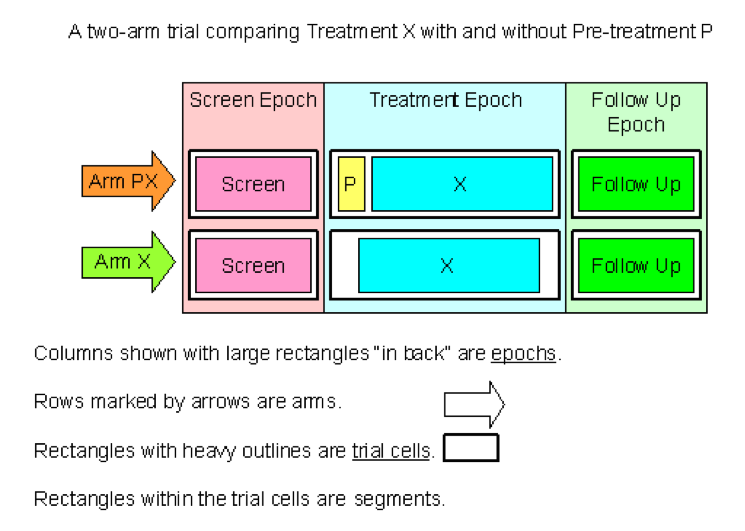
\includegraphics[width=\linewidth]{./CDISCTrialStructure}
\caption{Overview of the Trial Structure used in the CDISC Study
  Design Model.}
\label{fig:cdiscstruct}
\end{figure}


To get an idea how this works in practise, the following example shows
a simple clinical trial describing a steady state model, with one
study arm.

\begin{xmlcode}
    <TrialDesign xmlns="http://www.pharmml.org/2013/03/TrialDesign">
        <Structure>
            <!-- Define the trial structure -->
            <Epoch oid="e1">
                <Order>1</Order>
            </Epoch>
            <Arm oid="a1"/>
            <Cell oid="c1">
                <EpochRef oid="e1"/>
                <ArmRef oid="a1"/>
                <SegmentRef oid="s1"/>
            </Cell>
            <Segment oid="s1">
                <ActivityRef oid="a1"/>
            </Segment>
            <Activity oid="a1">
                <Bolus>
                    <DoseAmount>
                        <DoseVar block="main" symbId="D"/>
                        <ct:Assign>
                            <ct:Real>100</ct:Real>
                        </ct:Assign>
                    </DoseAmount>
                    <SteadyState>
                        <EndTime>
                            <ct:SymbRef symbId="tD"/>
                            <ct:Assign><ct:Real>0</ct:Real></ct:Assign>
                        </EndTime>
                        <Interval>
                            <ct:SymbRef block="p1" symbId="tau"/>
                            <ct:Assign><ct:Real>12</ct:Real></ct:Assign>
                        </Interval>
                    </SteadyState>
                </Bolus>
            </Activity>
        </Structure>
        <Population>
            <!-- Define the variability level associated with the
            population -->
            <ct:VariabilityReference>
                <ct:SymbRef symbId=""></ct:SymbRef>
            </ct:VariabilityReference>
            <!-- Define the individuals -->
            <Individual oid="i">
                <ArmRef oid="a1"/>
                <Replicates>
                    <ct:Int>50</ct:Int>
                </Replicates>
            </Individual>
        </Population>
    </TrialDesign>
\end{xmlcode}

The CDISC like elements are contained in the \xelem{Structure}
tag and you can see how the study is constructed of a single epoch,
with a single arm and a single cell that contains a single
segment. Note, though that this structure is not hierarchical and the
\xelem{Cell} element joins together the arms, epoch and segments
together. Note that a Cell can span several arms contains several
segments. Finally the segment points to an activity the describes
the steady state dosing regimen. The dosing regimen is very similar
to that used in version 0.1 of \pharmml. The details should be ignored
here and please refer to proposed changes to the dosing regimen in the
section below.

Following on from the \xelem{Structure} element is
\xelem{Population}. This is where we describe the individuals in the
study, their attributes (such as weight, gender etc) and assign them
to an arm of the study. In this simple example we only have one arm
and so we assign all the individuals in the study to that arm. As a
shorthand we provide one individual definition and use the element
\xelem{Replicates} to specify how many individuals this
represents. This is obviously useful when simulating a model when (as
in this example) covariates such as weight are calculated for each
individual. An identifier for each individual is created on the fly by
suffixing a sequential number after the identifier. In this case they
would be i1, i2 \ldots i49, i50. While not useful at the moment, such
identifiers will be generated when writing out output to a file. The
\xelem{Replicates} element is optional and later examples will
enumerate the properties of each individual in the population without
using it.

In this simple example the same amount of dose was administered for
each individual. However, in many models the size of the dose varies
per individual. In the example below you can see more complex trial
design with multiple arms and dosing specified per individual. This
corresponds the trial design describing example 6 in the \pharmml
specification. I've reproduced the figure describing it below (figure
\ref{fig:eg6-trial-design}).

\begin{figure}[htb]
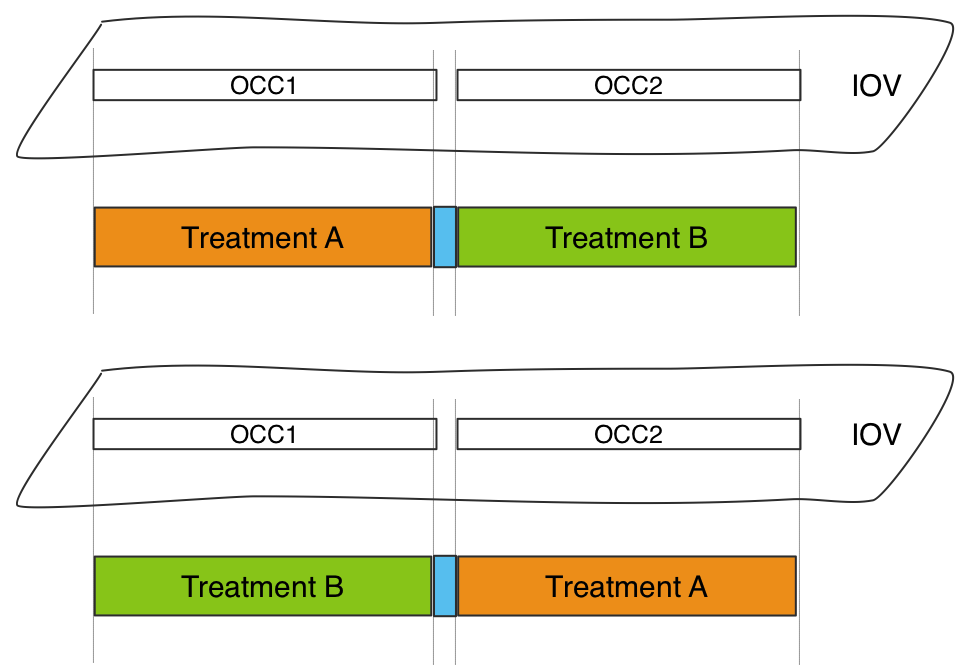
\includegraphics[width=\linewidth]{../pics/iov1simulation_grafio}
\caption{Overview of the trial design used in example 6 of the spec.}
\label{fig:eg6-trial-design}
\end{figure}

\begin{xmlcode}
    <TrialDesign xmlns="http://www.pharmml.org/2013/03/TrialDesign">
        <Structure>
            <Epoch oid="ep1">
                <Order>1</Order>
            </Epoch>
            <Epoch oid="ep2">
                <Order>2</Order>
            </Epoch>
            <Epoch oid="ep3">
                <Order>3</Order>
            </Epoch>
            <Arm oid="a1"/>
            <Arm oid="a2"/>
            <Cell oid="c1">
                <EpochRef oid="e1" />
                <ArmRef oid="a1"/>
                <SegmentRef oid="ta"/>
            </Cell>
            <Cell oid="c2">
                <EpochRef oid="e1" />
                <ArmRef oid="a1"/>
                <SegmentRef oid="tb"/>
            </Cell>
            <Cell oid="c3">
                <EpochRef oid="e2" />
                <ArmRef oid="a1"/>
                <ArmRef oid="a2"/>
                <SegmentRef oid="wash"/>
            </Cell>
            <Cell oid="c4">
                <EpochRef oid="e3"/>
                <ArmRef oid="a1"/>
                <SegmentRef oid="tb"/>
            </Cell>
            <Cell oid="c5">
                <EpochRef oid="e3"/>
                <ArmRef oid="a2"/>
                <SegmentRef oid="ta"/>
            </Cell>
            <Segment oid="ta">
                <ActivityRef oid="d1"/>
            </Segment>
            <Segment oid="tb">
                <ActivityRef oid="d2"/>
            </Segment>
            <Segment oid="wash">
                <ActivityRef oid="w1"/>
            </Segment>
            <Activity oid="d1">
                <Bolus>
                <!-- SNIP -->
                </Bolus>
            </Activity>
            <Activity oid="d2">
                <Bolus>
                <!-- SNIP -->
                </Bolus>
            </Activity>
            <Activity oid="w1">
                <Washout/>
            </Activity>
            <ObservationsEvent oid="occasions">
                <ArmRef oid="a1"/>
                <ArmRef oid="a2"/>
                <ct:VariabilityReference>
                    <ct:SymbRef block="model" symbId="iov"></ct:SymbRef>
                </ct:VariabilityReference>
                <ObservationGroup oid="occ1">
                    <EpochRef oid="ep1"/>
                </ObservationGroup>
                <ObservationGroup oid="occ2">
                    <EpochRef oid="ep3"/>
                </ObservationGroup>
            </ObservationsEvent>
        </Structure>
        <Population>
            <ct:VariabilityReference>
                <ct:SymbRef block="model" symbId="indiv"/>
            </ct:VariabilityReference>
            <Individual oid="i1">
                <ArmRef oid="a1"/>
                <Covariate>
                    <ct:SymbRef block="c1" symbId="Sex"/>
                    <ct:Assign><ct:String>M</ct:String></ct:Assign>
                </Covariate>
                <Covariate>
                    <ct:SymbRef block="c1" symbId="Treat"/>
                    <IVDependent>
                        <EpochRef oid="e1"/>
                        <ct:Assign>
                            <ct:String>A</ct:String>
                        </ct:Assign>
                    </IVDependent>
                    <IVDependent>
                        <EpochRef oid="e3"/>
                        <ct:Assign>
                            <ct:String>B</ct:String>
                        </ct:Assign>
                    </IVDependent>
                </Covariate>
            </Individual>
            <Individual oid="i2">
                <ArmRef oid="a1"/>
                <Covariate>
                    <ct:SymbRef block="c1" symbId="Sex"/>
                    <ct:Assign><ct:String>M</ct:String></ct:Assign>
                </Covariate>
                <Covariate>
                    <ct:SymbRef block="c1" symbId="Treat"/>
                    <IVDependent>
                        <EpochRef oid="e1"/>
                        <ct:Assign>
                            <ct:String>A</ct:String>
                        </ct:Assign>
                    </IVDependent>
                    <IVDependent>
                        <EpochRef oid="e3"/>
                        <ct:Assign>
                            <ct:String>B</ct:String>
                        </ct:Assign>
                    </IVDependent>
                </Covariate>
            </Individual>
            <Individual oid="i3">
                <!-- Omitted the remaining individual definitions
                for brevity -->
            </Individual>
        </Population>
    </TrialDesign>
\end{xmlcode}

In the above example you can see that the more complex trial design
structure is encoded, hopefully as you would expect. Note that the
washout is now defined clearly as an epoch. The new feature that was
not shown in the previous example is the definition of the
occasion as an ObservationsEvent. As you can see this enables us to
define a set of observations, and map them to a variability level. The
duration of each observation (specified by the
\xelem{ObservationGroup} element) can be defined as the duration of a
specified epoch (as in this example) or can be a time period. The
later only makes sense if the epochs define time periods
too\footnote{Note that if each epoch specifies a time period then an
  ObservationEvent can specify a time period that spans multiple
  epochs.}. The \xelem{ObservationsEvent} is associated with an arm,
which means that different sets of inter-occasion variability can be
applied to different arms. I'm not sure if this makes sense or whether
the \xelem{ObservationsEvent} should apply to all arm at the same time
--- and therefore all subjects in the study.

Note also that the definition of the population is richer, with
covariates being defined with each individual. In this example too
each individual in the study is being explicitly defined. Take
particular note of the \xelem{IVDependent} element which is a child of
the \xelem{Individual} element. This is how we define covariates that
are dependent on the independent variable (typically time). In this
example we specify a value for the covariate to be used during a given
epoch. However, it is also possible to specify a time-point
which specifies from which time in the study the covariate value applies.


Perhaps the most complex example is from the Chan and Holford
model\footnote{ref} that defines the most complex trial design
structure that we have so far encoded. It was only possible to encode
this using the data-file approach in the previous version of \pharmml
and even then we had to fix a problem where this method could not
define steady state dosing. As it stands this model cannot be encoded
in version 0.1 of \pharmml. The example is below:

\begin{xmlcode}
    <TrialDesign xmlns="http://www.pharmml.org/2013/03/TrialDesign">
        <Structure>
            <Epoch oid="m0">
                <Start>
                    <ct:Real>0</ct:Real>
                </Start>
                <End>
                    <ct:Real>90</ct:Real>
                </End>
                <Order>1</Order>
            </Epoch>
            <Epoch oid="m6">
                <Start>
                    <ct:Real>408</ct:Real>
                </Start>
                <End>
                    <ct:Real>499</ct:Real>
                </End>
                <Order>2</Order>
            </Epoch>
            <Epoch oid="m12">
                <Start>
                    <ct:Real>908</ct:Real>
                </Start>
                <End>
                    <ct:Real>9999</ct:Real>
                </End>
                <Order>3</Order>
            </Epoch>
            <Epoch oid="m24">
                <Start>
                    <ct:Real>1908</ct:Real>
                </Start>
                <End>
                    <ct:Real>1999</ct:Real>
                </End>
                <Order>4</Order>
            </Epoch>
            <Epoch oid="m48">
                <Start>
                    <ct:Real>3908</ct:Real>
                </Start>
                <End>
                    <ct:Real>3999</ct:Real>
                </End>
                <Order>5</Order>
            </Epoch>
            <Arm oid="a1"/>
            <Cell oid="c1">
                <EpochRef oid="m1"/>
                <ArmRef oid="a1"/>
                <SegmentRef oid="s1"/>
            </Cell>
            <Cell oid="c2">
                <EpochRef oid="m6"/>
                <ArmRef oid="a1"/>
                <SegmentRef oid="s2"/>
            </Cell>
            <Cell oid="c2">
                <EpochRef oid="m12"/>
                <ArmRef oid="a1"/>
                <SegmentRef oid="s2"/>
            </Cell>
            <Cell oid="c2">
                <EpochRef oid="m24"/>
                <ArmRef oid="a1"/>
                <SegmentRef oid="s2"/>
            </Cell>
            <Cell oid="c2">
                <EpochRef oid="m48"/>
                <ArmRef oid="a1"/>
                <SegmentRef oid="s2"/>
            </Cell>
            <Segment oid="s1">
                <ActivityRef oid="exoinf"/>
            </Segment>
            <Segment oid="s2">
                <ActivityRef oid="exoinf"/>
                <ActivityRef oid="oralss"/>
            </Segment>
            <Activity oid="exoinf">
                <Infusion>
                    <DoseAmount>
                        <TargetVar block="sm1" symbId="Ac"/>
                    </DoseAmount>
                    <DosingTimes>
                        <ct:Assign>
                            <ct:Vector>
                                <ct:Real>0</ct:Real>
                                <ct:Real>72</ct:Real>
                            </ct:Vector>
                        </ct:Assign>
                    </DosingTimes>
                    <Duration><ct:SymbRef block="pm1" symbId="TTK0"></ct:SymbRef></Duration>
                </Infusion>
            </Activity>
            <Activity oid="oralss">
                <Infusion>
                    <DoseAmount>
                        <TargetVar block="sm1" symbId="Ac"/>
                        <ct:Assign><ct:SymbRef block="pm1" symbId="Css"/></ct:Assign>
                    </DoseAmount>
                    <SteadyState>
                        <EndTime>
                            <ct:Assign>
                                <ct:Real>0</ct:Real>
                            </ct:Assign>
                        </EndTime>
                    </SteadyState>
                    <Rate><ct:SymbRef block="sm1" symbId="R1"></ct:SymbRef></Rate>
                </Infusion>
            </Activity>
            <ObservationsEvent oid="occ">
                <ArmRef oid="a1"/>
                <ct:Name>Occasions</ct:Name>
                <ct:VariabilityReference>
                    <ct:SymbRef symbId="occ"/>
                </ct:VariabilityReference>
                <ObservationGroup oid="occ1">
                   <Period> <Start>
                        <ct:Real>0</ct:Real>
                    </Start>
                    <End>
                        <ct:Real>24</ct:Real>
                    </End></Period>
                </ObservationGroup>
                <ObservationGroup oid="occ2">
                    <Period><Start>
                        <ct:Real>72</ct:Real>
                    </Start>
                    <End>
                        <ct:Real>90</ct:Real>
                    </End></Period>
                </ObservationGroup>
                <ObservationGroup oid="occ3">
                    <Period><Start>
                        <ct:Real>408</ct:Real>
                    </Start>
                    <End>
                        <ct:Real>457</ct:Real>
                    </End></Period>
                </ObservationGroup>
                <ObservationGroup oid="occ4">
                    <Period><Start>
                        <ct:Real>481</ct:Real>
                    </Start>
                    <End>
                        <ct:Real>499</ct:Real>
                    </End></Period>
                </ObservationGroup>
                <ObservationGroup oid="occ5">
                   <Period> <Start>
                        <ct:Real>908</ct:Real>
                    </Start>
                    <End>
                        <ct:Real>957</ct:Real>
                    </End></Period>
                </ObservationGroup>
                <ObservationGroup oid="occ6">
                    <Period><Start>
                        <ct:Real>981</ct:Real>
                    </Start>
                    <End>
                        <ct:Real>999</ct:Real>
                    </End></Period>
                </ObservationGroup>
                <ObservationGroup oid="occ7">
                    <Period><Start>
                        <ct:Real>1908</ct:Real>
                    </Start>
                    <End>
                        <ct:Real>1957</ct:Real>
                    </End></Period>
                </ObservationGroup>
                <ObservationGroup oid="occ8">
                   <Period> <Start>
                        <ct:Real>1981</ct:Real>
                    </Start>
                    <End>
                        <ct:Real>1999</ct:Real>
                    </End></Period>
                </ObservationGroup>
                <ObservationGroup oid="occ9">
                    <Period><Start>
                        <ct:Real>3908</ct:Real>
                    </Start>
                    <End>
                        <ct:Real>3957</ct:Real>
                    </End></Period>
                </ObservationGroup>
                <ObservationGroup oid="occ10">
                    <Period><Start>
                        <ct:Real>3981</ct:Real>
                    </Start>
                    <End>
                        <ct:Real>3999</ct:Real>
                    </End></Period>
                </ObservationGroup>
            </ObservationsEvent>
            <ObservationsEvent oid="trial">
                <ArmRef oid="a1"/>
                <ct:Name>Trials</ct:Name>
                <ct:VariabilityReference>
                    <ct:SymbRef symbId="occ"/>
                </ct:VariabilityReference>
                <ObservationGroup oid="t1">
                    <EpochRef oid="m1"/>
                </ObservationGroup>
                <ObservationGroup oid="t1">
                    <EpochRef oid="m6"/>
                </ObservationGroup>
                <ObservationGroup oid="t1">
                    <EpochRef oid="m12"/>
                </ObservationGroup>
                <ObservationGroup oid="t4">
                    <EpochRef oid="m24"/>
                </ObservationGroup>
                <ObservationGroup oid="t5">
                    <EpochRef oid="m48"/>
                </ObservationGroup>
            </ObservationsEvent>
        </Structure>
        <Population>
            <ct:VariabilityReference>
                <ct:SymbRef symbId=""/>
            </ct:VariabilityReference>
            <Individual oid="i552">
                <ArmRef oid="a1"/>
                <Covariate>
                    <ct:SymbRef block="c1" symbId="W"/>
                    <IVDependent>
                        <EpochRef oid="m1"/>
                        <ct:Assign><ct:Real>73</ct:Real></ct:Assign>
                    </IVDependent>
                    <IVDependent>
                        <EpochRef oid="m6"/>
                        <ct:Assign><ct:Real>70</ct:Real></ct:Assign>
                    </IVDependent>
                    <IVDependent>
                        <EpochRef oid="m12"/>
                        <ct:Assign><ct:Real>73</ct:Real></ct:Assign>
                    </IVDependent>
                    <IVDependent>
                        <EpochRef oid="m24"/>
                        <ct:Assign><ct:Real>71</ct:Real></ct:Assign>
                    </IVDependent>
                    <IVDependent>
                        <EpochRef oid="m48"/>
                        <ct:Assign><ct:Real>69</ct:Real></ct:Assign>
                    </IVDependent>
                </Covariate>
            </Individual>
        </Population>
        <IndividualDosing>
                <ActivityRef oid="inf1"/>
                <Individual columnRef="id"/>
                <DoseAmount columnRef="dose"/>
                <DosingTime columnRef="t"/>
                <DataSet xmlns="http://www.pharmml.org/2013/03/CommonTypes">
                    <Definition>
                        <Column columnNum="1" columnVar="id"/>
                        <Column columnNum="2" columnVar="t"/>
                        <Column columnNum="3" columnVar="dose"/>
                    </Definition>
                    <Row>
                        <String>i552</String><Real>0</Real><Real>740.37</Real>
                        <String>i552</String><Real>72</Real><Real>740.37</Real>
                        <String>i552</String><Real>409</Real><Real>709.94</Real>
                        <String>i552</String><Real>481</Real><Real>709.94</Real>
                        <String>i552</String><Real>909</Real><Real>740.94</Real>
                        <String>i552</String><Real>981</Real><Real>740.94</Real>
                        <String>i552</String><Real>1909</Real><Real>720.08</Real>
                        <String>i552</String><Real>1981</Real><Real>720.08</Real>
                        <String>i552</String><Real>3909</Real><Real>699.8</Real>
                        <String>i552</String><Real>3981</Real><Real>699.8</Real>
                    </Row>
                </DataSet>
        </IndividualDosing>
    </TrialDesign>
\end{xmlcode}

This uses all the components that you have seen in the previous
examples, with the addition of the \xelem{IndividualDosing}
element. Its purpose is to provide per individual dosing information
a given dosing activity (specified by \verb|<ActivityRef oid="inf1"/>|).
Note that in this example the dose varies with time, but of course it
need not do, in which case the time column and \xelem{DosingTime}
record are omitted. Note that the type of each value is specified
explicitly so it is clear whether the value is compatible with the
information it is being mapped to. If we need dosing information for
more than one dosing activity then multiple \xelem{IndividualDosing}
can be defined.

\section{Simplifying the Estimation and Simulation Steps}

A by-product of the redesign of the Trial Design structure is that the
estimation and simulation steps can be considerably
simplified. Perhaps the greatest simplification is with the
\xelem{SimulationStep} which can drop the need to specify the design
in a data file. It now just needs to define initial values and specify
what observations to simulate. A by-product of the re-design is that
we also fix one of the unresolved issues in version 0.1 of
\pharmml. It wasn't clear how to simulate only one epoch since it was
possible for each epoch to have the same time period when separated by
a washout. Now however the epochs must specify consecutive time
periods so the simulation can easily be defined to span all the time
periods in all the epochs of the study.

Finally the use of a data-file in the estimation step becomes very
simple. See for example the estimation step of the Holford and Chan
model:
%
\begin{xmlcode}
<EstimationStep id="estTask1">
    <ObjectiveDataSet>
        <IndividualMapping>
            <ColumnRef oid="id"/>
        </IndividualMapping>
        <VariableMapping>
            <ColumnRef oid="time"/>
            <ct:SymbRef symbId="t"/>
            <Interpolation>
                <Method name="default"/>
            </Interpolation>
        </VariableMapping>
        <VariableMapping>
            <ColumnRef oid="DV"/>
            <ct:SymbRef block="om1" symbId="CP"></ct:SymbRef>
            <Interpolation>
                <Method name="default"/>
            </Interpolation>
        </VariableMapping>
        <ct:DataSet>
            <ct:Definition>
                <ct:Column columnNum="1" columnVar="id"/>
                <ct:Column columnNum="2" columnVar="time"/>
                <ct:Column columnNum="3" columnVar="DV"/>
            </ct:Definition>
            <ct:Row>
                <ct:String>i552</ct:String><ct:Real>0</ct:Real><ct:Real>0.46</ct:Real>
                <ct:String>i552</ct:String><ct:Real>1</ct:Real><ct:Real>6.11</ct:Real>
                <ct:String>i552</ct:String><ct:Real>1.5</ct:Real><ct:Real>7.38</ct:Real>
                <ct:String>i552</ct:String><ct:Real>2</ct:Real><ct:Real>7.73</ct:Real>
                <!-- Snip -->
            </ct:Row>
        </ct:DataSet>
    </ObjectiveDataSet>
    <ParametersToEstimate>
      <!-- Snip -->
    </ParametersToEstimate>
    <EstimationOperation opType="estPop"/>
</EstimationStep>
\end{xmlcode}
%
Here the mapping of the objective data to the model becomes trivial and
this simplicity enables us to focus on issues we neglected when the
\xelem{EstimationStep} was more complicated. You will notice that each
\xelem{VariableMapping} element contains an \xelem{Interpolation}
element. This allows us to specify how the data should be interpolated
during the estimation procedure. The only available method at the
moment is \emph{default} so clearly this needs more work, but the
objective is clear.

We can extend this approach to also support multiple datasets within
one estimation step. Why? Well possible scenarios are:
\begin{enumerate}
\item You have separate PK and PD measurements taken at different
  time-points.
\item You have replicate observations and you want to map each
  replicate to a different error model.
\end{enumerate}
The hypothetical example below shows, how you might describe the first
case:
\begin{xmlcode}
<EstimationStep id="estTask1">
    <ObjectiveDataSet>
        <IndividualMapping>
            <ColumnRef oid="id"/>
        </IndividualMapping>
        <VariableMapping>
            <ColumnRef oid="time"/>
            <ct:SymbRef symbId="t"/>
            <Interpolation>
                <Method name="default"/>
            </Interpolation>
        </VariableMapping>
        <VariableMapping>
            <ColumnRef oid="DV"/>
            <ct:SymbRef block="om1" symbId="Cc"></ct:SymbRef>
            <Interpolation>
                <Method name="default"/>
            </Interpolation>
        </VariableMapping>
        <ct:DataSet>
            <ct:Definition>
                <ct:Column columnNum="1" columnVar="id"/>
                <ct:Column columnNum="2" columnVar="time"/>
                <ct:Column columnNum="3" columnVar="DV"/>
            </ct:Definition>
            <ct:Row>
                <ct:String>i1</ct:String><ct:Real>0</ct:Real><ct:Real>0</ct:Real>
                <ct:String>i1</ct:String><ct:Real>1</ct:Real><ct:Real>5</ct:Real>
                <ct:String>i1</ct:String><ct:Real>4</ct:Real><ct:Real>9</ct:Real>
                <ct:String>i1</ct:String><ct:Real>6</ct:Real><ct:Real>11</ct:Real>
                <!-- Snip -->
            </ct:Row>
        </ct:DataSet>
    </ObjectiveDataSet>
    <ObjectiveDataSet>
        <IndividualMapping>
            <ColumnRef oid="id"/>
        </IndividualMapping>
        <VariableMapping>
            <ColumnRef oid="time"/>
            <ct:SymbRef symbId="t"/>
            <Interpolation>
                <Method name="default"/>
            </Interpolation>
        </VariableMapping>
        <VariableMapping>
            <ColumnRef oid="DV"/>
            <ct:SymbRef block="om1" symbId="E"></ct:SymbRef>
            <Interpolation>
                <Method name="default"/>
            </Interpolation>
        </VariableMapping>
        <ct:DataSet>
            <ct:Definition>
                <ct:Column columnNum="1" columnVar="id"/>
                <ct:Column columnNum="2" columnVar="time"/>
                <ct:Column columnNum="3" columnVar="DV"/>
            </ct:Definition>
            <ct:Row>
                <ct:String>i1</ct:String><ct:Real>0</ct:Real><ct:Real>0</ct:Real>
                <ct:String>i1</ct:String><ct:Real>6</ct:Real><ct:Real>0</ct:Real>
                <ct:String>i1</ct:String><ct:Real>12</ct:Real><ct:Real>10</ct:Real>
                <ct:String>i1</ct:String><ct:Real>24</ct:Real><ct:Real>20</ct:Real>
                <ct:String>i1</ct:String><ct:Real>36</ct:Real><ct:Real>40</ct:Real>
                <ct:String>i1</ct:String><ct:Real>48</ct:Real><ct:Real>80</ct:Real>
                <!-- Snip -->
            </ct:Row>
        </ct:DataSet>
    </ObjectiveDataSet>
    <ParametersToEstimate>
      <!-- Snip -->
    </ParametersToEstimate>
    <EstimationOperation opType="estPop"/>
</EstimationStep>
\end{xmlcode}
%
Here as you can see there are two datasets. The first provides
measurements for the PK variable $\mathrm{Cc}$ and the second for the
effect variable $E$. The example below shows the second case where the
first dataset describes the first set of replicates and the second
dataset the other. Note that we indicate to the observation model
which replicate set it is being assigning a value to an indicator variable.
%
\begin{xmlcode}
<EstimationStep id="estTask1">
    <ObjectiveDataSet>
        <IndividualMapping>
            <ColumnRef oid="id"/>
        </IndividualMapping>
        <ct:VariableAssignment>
            <ct:SymbRef symbId="replicateFlag"/>
            <ct:Assign>
                <ct:Int>1</ct:Int>
            </ct:Assign>
        </ct:VariableAssignment>
        <VariableMapping>
            <ColumnRef oid="time"/>
            <ct:SymbRef symbId="t"/>
            <Interpolation>
                <Method name="default"/>
            </Interpolation>
        </VariableMapping>
        <VariableMapping>
            <ColumnRef oid="DV"/>
            <ct:SymbRef block="om1" symbId="Cc"></ct:SymbRef>
            <Interpolation>
                <Method name="default"/>
            </Interpolation>
        </VariableMapping>
        <ct:DataSet>
            <!-- Snip -->
        </ct:DataSet>
    </ObjectiveDataSet>
    <ObjectiveDataSet>
        <IndividualMapping>
            <ColumnRef oid="id"/>
        </IndividualMapping>
        <ct:VariableAssignment>
            <ct:SymbRef symbId="replicateFlag"/>
            <ct:Assign>
                <ct:Int>2</ct:Int>
            </ct:Assign>
        </ct:VariableAssignment>
        <VariableMapping>
            <ColumnRef oid="time"/>
            <ct:SymbRef symbId="t"/>
            <Interpolation>
                <Method name="default"/>
            </Interpolation>
        </VariableMapping>
        <VariableMapping>
            <ColumnRef oid="DV"/>
            <ct:SymbRef block="om1" symbId="Cc"></ct:SymbRef>
            <Interpolation>
                <Method name="default"/>
            </Interpolation>
        </VariableMapping>
        <ct:DataSet>
            <!-- Snip -->
        </ct:DataSet>
    </ObjectiveDataSet>
    <ParametersToEstimate>
      <!-- Snip -->
    </ParametersToEstimate>
    <EstimationOperation opType="estPop"/>
</EstimationStep>
\end{xmlcode}
% 
Because we can duplicate datasets in this way this allows us to add a
constraint on the datasets we can use. Namely that we only allow one 
row per combination of individual and time. In doing so we can
then permit observations to be defined in an order independent
way. So:
%
\begin{xmlcode}
<ct:Row>
    <ct:String>i1</ct:String><ct:Real>0</ct:Real><ct:Real>0</ct:Real>
    <ct:String>i1</ct:String><ct:Real>6</ct:Real><ct:Real>0</ct:Real>
    <ct:String>i1</ct:String><ct:Real>12</ct:Real><ct:Real>10</ct:Real>
    <ct:String>i1</ct:String><ct:Real>24</ct:Real><ct:Real>20</ct:Real>
    <ct:String>i1</ct:String><ct:Real>36</ct:Real><ct:Real>40</ct:Real>
    <ct:String>i1</ct:String><ct:Real>48</ct:Real><ct:Real>80</ct:Real>
    <!-- Snip -->
</ct:Row>
\end{xmlcode}
%
is therefore equivalent to:
\begin{xmlcode}
<ct:Row>
    <ct:String>i1</ct:String><ct:Real>48</ct:Real><ct:Real>80</ct:Real>
    <ct:String>i1</ct:String><ct:Real>12</ct:Real><ct:Real>10</ct:Real>
    <ct:String>i1</ct:String><ct:Real>24</ct:Real><ct:Real>20</ct:Real>
    <ct:String>i1</ct:String><ct:Real>0</ct:Real><ct:Real>0</ct:Real>
    <ct:String>i1</ct:String><ct:Real>6</ct:Real><ct:Real>0</ct:Real>
    <ct:String>i1</ct:String><ct:Real>36</ct:Real><ct:Real>40</ct:Real>
    <!-- Snip -->
</ct:Row>
\end{xmlcode}
%
Remember that this representation is meant for information exchange
between software tools. For a human reader this may seem more complex
to comprehend, but for software the fact that there are no duplicates
and no order makes the processing and validation of this information
less so.

\end{document}
